%%%%%%%%%%%%%%%%%%%%%%%%%%%%%%%%%%%%%%%%%%%%%%%%%%%%%%%%%%%%%%%%%%%%
\section{Relic density -- theoretical background}

\subsection{The Boltzmann equation and thermal averaging}
\label{sec:Boltzmann}

Griest and Seckel \cite{GriestSeckel} have worked out the Boltzmann
equation when coannihilations are included. We start by reviewing
their expressions and then continue by rewriting them into a more
convenient form that resembles the familiar case without
coannihilations. This allows us to use similar expressions for
calculating thermal averages and solving the Boltzmann equation
whether coannihilations are included or not. The implementation in
\ds\ is based upon the work done in \cite{edsjo97}. We will later in this
chapter, for the sake of clarification, assume that we work with
supersymmetric dark matter with the lightest neutralino being the
LSP. The routines here are completely general though and the interface
between supersymmetry and the relic density routines is handled by the
routines in \codeb{src/rn}.


\subsection{Review of the Boltzmann equation with coannihilations}

Consider annihilation of $N$ supersymmetric particles $\chi_i$
($i=1,\ldots,N$) with masses $m_i$ and internal degrees of freedom
(statistical weights) $g_i$.  Also assume that $m_1 \leq m_2 \leq
\cdots \leq m_{N-1} \leq m_N$ and that $R$-parity is conserved. Note
that for the mass of the lightest neutralino we will use the
notation $m_{\chi}$ and $m_{1}$ interchangeably.

The evolution of the number density $n_i$ of particle $i$ is
\begin{eqnarray} \label{eq:Boltzmann}
  \frac{dn_{i}}{dt} 
  &=& 
  -3 H n_{i} 
  - \sum_{j=1}^N \langle \sigma_{ij} v_{ij} \rangle 
    \left( n_{i} n_{j} - n_{i}^{\rm{eq}} n_{j}^{\rm{eq}} \right) 
  \nonumber \\ 
  & & 
  - \sum_{j\ne i} 
  \big[ \langle \sigma'_{Xij} v_{ij} \rangle 
        \left( n_i n_X - n_{i}^{\rm{eq}} n_{X}^{\rm{eq}} \right)
      - \langle \sigma'_{Xji} v_{ij} \rangle
        \left( n_j n_X - n_{j}^{\rm{eq}} n_{X}^{\rm{eq}} \right)
  \big]
  \nonumber \\ 
  & &
  - \sum_{j\ne i} 
  \big[ \Gamma_{ij} 
        \left( n_i - n_i^{\rm{eq}} \right) 
      - \Gamma_{ji} 
        \left( n_j - n_j^{\rm{eq}} \right) 
  \big] .
\end{eqnarray}
The first term on the right-hand side is the dilution due to the
expansion of the Universe. $H$ is the Hubble parameter. The second
term describes $\chi_i\chi_j$ annihilations, whose total
annihilation cross section is 
\begin{eqnarray}
  \sigma_{ij}  & = & \sum_X \sigma (\chi_i \chi_j \rightarrow X).
\end{eqnarray}
The third term describes $\chi_i \to \chi_j$ conversions by
scattering off the cosmic thermal background,
\begin{eqnarray}
  \sigma'_{Xij} & = & \sum_Y \sigma (\chi_i X \rightarrow \chi_j Y)
\end{eqnarray}
being the inclusive scattering cross section. The last term accounts
for $\chi_i$ decays, with inclusive decay rates 
\begin{eqnarray}
  \Gamma_{ij}  & = & \sum_X \Gamma (\chi_i \rightarrow \chi_j X).
\end{eqnarray}
In the previous expressions, $X$ and $Y$
are (sets of) standard model particles involved in the
interactions, $v_{ij}$ is the `relative velocity' defined by
\begin{equation}
  v_{ij} = \frac{\sqrt{(p_{i} \cdot p_{j})^2-m_{i}^2 m_{j}^2}}{E_{i} E_{j}}
\end{equation}
with $p_{i}$ and $E_{i}$ being the four-momentum and energy of 
particle $i$, and finally $n_{i}^{\rm{eq}}$ is the equilibrium number
density of particle $\chi_i$,
\begin{equation}
  n_{i}^{\rm{eq}} = \frac{g_{i}}{(2\pi)^3} \int d^3{\bf p}_{i}f_{i}
\end{equation}
where ${\bf p}_i$ is the three-momentum of particle $i$, and
 $f_i$ is its equilibrium distribution function. 
In the Maxwell-Boltzmann approximation it is given by
\begin{equation}
  f_{i} = e^{-E_{i}/T}.
\end{equation}
The thermal average $\langle\sigma_{ij}v_{ij}\rangle$ is defined
with equilibrium distributions and is given by
\begin{equation}
  \langle \sigma_{ij}v_{ij} \rangle = \frac{\int d^3{\bf
      p}_{i}d^3{\bf p}_{j} 
  f_{i}f_{j}\sigma_{ij}v_{ij}}
  {\int d^3{\bf p}_{i}d^3{\bf p}_{j}f_{i}f_{j}}
\end{equation}

Normally, the decay rate of supersymmetric particles $\chi_i$ other
than the lightest which is stable is much faster than the age of the
universe. Since we have assumed $R$-parity conservation, all of these
particles decay into the lightest one. So its final abundance is
simply described by the sum of the density of all supersymmetric
particles,
\begin{equation}
  n= \sum_{i=1}^N n_{i}.
\end{equation}
For $n$ we get the following evolution equation
\begin{equation}
  \frac{dn}{dt} = -3Hn - \sum_{i,j=1}^N \langle \sigma_{ij} v_{ij} \rangle 
  \left( n_{i}n_{j} - n_{i}^{\rm{eq}}n_{j}^{\rm{eq}} \right)
\end{equation}
where the terms on the second and third lines in
Eq.~(\ref{eq:Boltzmann}) cancel in the sum. 

The scattering rate of supersymmetric particles off particles in the
thermal background is much faster than their annihilation rate,
because the scattering cross sections $\sigma'_{Xij}$ are of the same
order of magnitude as the annihilation cross sections $\sigma_{ij}$
but the background particle density $n_X$ is much larger than each of
the supersymmetric particle densities $n_i$ when the former are
relativistic and the latter are non-relativistic, and so suppressed by
a Boltzmann factor. In this case, the $\chi_i$ distributions remain in
thermal equilibrium, and in particular their ratios are equal to the
equilibrium values,
\begin{equation}
  \frac{n_{i}}{n} \simeq \frac{n_{i}^{\rm{eq}}}{n^{\rm{eq}}}.
\end{equation}
We then get
\begin{equation} \label{eq:Boltzmann2}
  \frac{dn}{dt} =
  -3Hn - \langle \sigma_{\rm{eff}} v \rangle 
  \left( n^2 - n_{\rm{eq}}^2 \right)
\end{equation}
where
\begin{equation} \label{eq:sigmaveffdef}
  \langle \sigma_{\rm{eff}} v \rangle = \sum_{ij} \langle
  \sigma_{ij}v_{ij} \rangle \frac{n_{i}^{\rm{eq}}}{n^{\rm{eq}}}
  \frac{n_{j}^{\rm{eq}}}{n^{\rm{eq}}}.
\end{equation}

%%%%%%%%%%%%%%%%%

\subsection{Thermal averaging}
\label{sec:thermav}

So far the reviewing. Now let's continue
by reformulating the thermal averages into
more convenient expressions. 

We rewrite Eq.~(\ref{eq:sigmaveffdef}) as
\begin{equation} \label{eq:sigmaveff}
  \langle \sigma_{\rm{eff}} v \rangle = \frac{ \sum_{ij} \langle
  \sigma_{ij}v_{ij} \rangle n_{i}^{\rm{eq}} n_{j}^{\rm{eq}}}{n^2_{\rm{eq}}}
  = 
  \frac{A}{n_{\rm{eq}}^2} \, .
\end{equation}

For the denominator we obtain, 
using Boltzmann statistics for $f_i$,
\begin{equation} \label{eq:neq}
  n^{\rm eq} = \sum_i n^{\rm eq}_i = 
  \sum_i \frac{g_i}{(2\pi)^3} \int d^3 p_i 
  e^{-E_{i}/T} = 
  \frac{T}{2\pi^2} \sum_i g_i m_{i}^2
  K_{2} \left( \frac{m_{i}}{T}\right)
\end{equation}
where $K_{2}$ is the modified Bessel function of the second kind of 
order 2.

The numerator is the total annihilation rate per unit volume
at temperature $T$,
\begin{equation} 
  A = \sum_{ij} \langle \sigma_{ij} v_{ij} \rangle n_i^{\rm eq}
  n_j^{\rm eq} = \sum_{ij} \frac{g_{i}g_{j}}{(2\pi)^6} \int d^3 {\bf p}_{i}
  d^3{\bf p}_{j} f_{i}f_{j} \sigma_{ij} v_{ij}
\end{equation}
It is convenient
to cast it in a covariant form,
\begin{equation} 
  A = \sum_{ij} 
  \int W_{ij} \frac{g_i f_i d^3{\bf p}_i}{(2\pi)^3 2E_i}
  \frac{g_j f_j d^3{\bf p}_j}{(2\pi)^3 2E_j} .
\label{eq:Aij2}
\end{equation}
$W_{ij}$ is the (unpolarized) annihilation rate per unit volume
corresponding to the covariant normalization of $2E$ colliding
particles per unit volume. $W_{ij}$ is a dimensionless Lorentz
invariant, related to the (unpolarized) cross section
through\footnote{The quantity $w_{ij}$ in Ref.\ \protect\cite{SWO}
  is $W_{ij}/4$.}
\begin{equation} \label{eq:Wijcross}
  W_{ij} = 4 p_{ij} \sqrt{s} \sigma_{ij} = 4 \sigma_{ij} \sqrt{(p_i
\cdot p_j)^2 - m_i^2 m_j^2} = 4 E_{i} E_{j} \sigma_{ij} v_{ij} .
\end{equation}
Here
\begin{equation}
  p_{ij} =
\frac{\left[s-(m_i+m_j)^2\right]^{1/2}
\left[s-(m_i-m_j)^2\right]^{1/2}}{2\sqrt{s}}
\end{equation}
is the momentum of particle $\chi_i$ (or $\chi_j$) in the
center-of-mass frame of the pair $\chi_i\chi_j$.

Averaging over initial and summing over final internal states, the
contribution to $W_{ij}$ of a general $n$-body final state is
\begin{equation}
  W^{n\rm{-body}}_{ij} = 
  \frac{1}{g_i g_j S_f} \sum_{\rm{internal~d.o.f.}} 
  \int  \left| {\cal M} \right|^2 (2\pi)^4 
\delta^4(p_i+p_j-{\textstyle \sum_f}p_f) \prod_f
   \frac{d^3{\bf p}_f}{(2\pi)^3 2E_f} , 
\end{equation}
where $S_f$ is a symmetry factor accounting for identical final state
particles (if there are $K$ sets of $N_k$ identical particles,
$k=1,\dots,K$, then $S_f = \prod_{k=1}^{K} N_k!$).  In particular, 
the contribution
of a two-body final state can be written as
\begin{equation}
  W^{\rm{2-body}}_{ij\to kl} = \frac{p_{kl}}{16\pi^2 g_i g_j S_{kl} \sqrt{s}}
  \sum_{\rm{internal~d.o.f.}} \int \left| {\cal M}(ij\to kl) \right|^2
  d\Omega ,
\end{equation}
where $p_{kl}$ is the final center-of-mass momentum, $S_{kl}$ is a
symmetry factor equal to 2 for identical final particles and to 1
otherwise, and the integration is over the outgoing directions of
one of the final particles.  As usual, an average over initial
internal degrees of freedom is performed.

We now reduce the integral in the covariant expression for $A$,
Eq.~(\ref{eq:Aij2}), from 6 dimensions to 1.
Using Boltzmann statistics for $f_i$ (a good approximation for
$T\lsim m$)
\begin{equation} \label{eq:Aij2b}
  A =
  \sum_{ij} \int g_i g_j W_{ij} e^{-E_{i}/T} e^{-E_{j}/T} 
\frac{d^3{\bf p}_i}{(2\pi)^3 2E_i}
  \frac{d^3{\bf p}_j}{(2\pi)^3 2E_j} ,
\end{equation}
where ${\bf p}_{i}$ and ${\bf p}_{j}$ are the three-momenta and
$E_{i}$ and $E_{j}$ are the energies of the colliding particles.
Following the procedure in Ref.~\cite{GondoloGelmini} we then rewrite
the momentum volume element as
\begin{equation}
  d^3 {\bf p}_{i} d^3 {\bf p}_{j} = 4 \pi |{\bf p}_{i}| E_i dE_{i}
  \, 4 \pi |{\bf p}_{j}| E_j dE_{j} \, \frac{1}{2} d \cos \theta
\end{equation}
where $\theta$ is the angle between ${\bf p}_{i}$ and 
${\bf p}_{j}$. Then we change integration variables from 
$E_{i}$, $E_{j}$, $\theta$ to $E_{+}$, $E_{-}$ and $s$, given by
\begin{equation}
  \left\{ \begin{array}{lcl}
  E_{+} & = & E_{i}+E_{j} \\
  E_{-} & = & E_{i}-E_{j} \\
  s & = & m_{i}^2+m_{j}^2 + 2E_{i}E_{j}-2 |{\bf p}_{i}| |{\bf
    p}_{j}| \cos \theta,
  \end{array} \right.
\end{equation}
whence the volume element becomes
\begin{equation}
  \frac{d^3{\bf p}_i}{(2\pi)^3 2E_i} \frac{d^3{\bf p}_j}{(2\pi)^3 2E_j} =
  \frac{1}{(2\pi)^4} \frac{dE_{+}dE_{-}ds}{8},
\end{equation}
and the integration region $\{ E_i \geq m_i, E_j \geq m_j, |\cos \theta| 
\leq
1\}$ transforms into 
\begin{eqnarray}
  && s \geq (m_i+m_j)^2, \\ && E_{+} \geq \sqrt{s} , \\ && \left\vert
  E_{-} - E_{+} \frac{m_j^2-m_i^2}{s} \right\vert \leq 2 p_{ij}
  \sqrt{\frac{E_{+}^2-s}{s}}.
\end{eqnarray}

Notice now that the product of the equilibrium distribution
functions depends only on $E_{+}$ and not $E_{-}$ due to the
Maxwell-Boltzmann approximation, and that the invariant rate
$W_{ij}$ depends only on $s$ due to the neglect of final state
statistical factors. Hence we can immediately integrate over
$E_{-}$,
\begin{equation}
  \int dE_{-} = 4p_{ij} \sqrt{\frac{E_{+}^2-s}{s}}.
\end{equation}
The volume element is now
\begin{equation}
  \frac{d^3{\bf p}_i}{(2\pi)^3 2E_i} \frac{d^3{\bf p}_j}{(2\pi)^3 2E_j} = 
  \frac{1}{(2\pi)^4} \frac{p_{ij}}{2} \sqrt{\frac{E_{+}^2-s}{s}} 
dE_{+} ds 
\end{equation}

We now perform the $E_{+}$ integration. We obtain
\begin{equation}
\label{eq:As}
  A = \frac{T}{32 \pi^4} \sum_{ij} \int_{(m_i+m_j)^2}^\infty ds
  g_ig_jp_{ij} W_{ij} K_{1} \left( \frac{\sqrt{s}}{T}\right)
\end{equation}
where $K_{1}$ is the modified Bessel function of the second kind of 
order 1.

We can take the sum inside the integral and define an effective
annihilation rate $W_{\rm eff}$ through
\begin{equation}
  \sum_{ij} g_i g_j p_{ij} W_{ij} = g_1^2 p_{\rm{eff}} W_{\rm{eff}}
\end{equation}
with
\begin{equation}
\label{eq:peff}
  p_{\rm{eff}} = p_{11} = \frac{1}{2} \sqrt{s-4m_{1}^2} .
\end{equation}
In other words
\begin{equation} \label{eq:weff}
  W_{\rm{eff}} = \sum_{ij}\frac{p_{ij}}{p_{11}}
  \frac{g_ig_j}{g_1^2} W_{ij} = 
  \sum_{ij} \sqrt{\frac{[s-(m_{i}-m_{j})^2][s-(m_{i}+m_{j})^2]}
  {s(s-4m_1^2)}} \frac{g_ig_j}{g_1^2} W_{ij}.
\end{equation}
Because $W_{ij}(s) = 0 $ for $s \le (m_i+m_j)^2$, the radicand is  
never negative.

In terms of cross sections, this is equivalent to the definition
\begin{equation}
\sigma_{\rm eff} = \sum_{ij} \frac{p^2_{ij}}{p^2_{11}}
  \frac{g_ig_j}{g_1^2} \sigma_{ij}.
\end{equation}  

Eq.~(\ref{eq:As}) then reads
\begin{equation}
  A = \frac{g_1^2 T}{32 \pi^4} \int_{4m_1^2}^\infty ds
  p_{\rm eff} W_{\rm eff} K_{1} \left( \frac{\sqrt{s}}{T}\right)
\end{equation}
This can be written in a form more suitable
for numerical integration by using $p_{\rm{eff}}$ instead of $s$ as
integration variable.  From Eq.~(\ref{eq:peff}), we have 
 $ ds = 8 p_{\rm{eff}} dp_{\rm{eff}} $, and 
\begin{equation}
\label{eq:Apeff}
  A = \frac{g_1^2 T}{4 \pi^4} \int_{0}^\infty dp_{\rm eff}
  p^2_{\rm eff} W_{\rm eff} K_{1} 
  \left( \frac{\sqrt{s}}{T}\right)
\end{equation}
with
\begin{equation}
  s = 4p_{\rm{eff}}^2 + 4m_1^2
\end{equation}
So we have succeeded in rewriting $A$ as a 1-dimensional integral.

{}From Eqs.~(\ref{eq:Apeff}) and~(\ref{eq:neq}), the thermal average of
the effective cross section results
\begin{equation} \label{eq:sigmavefffin2}
  \langle \sigma_{\rm{eff}}v \rangle = \frac{\int_0^\infty
  dp_{\rm{eff}} p_{\rm{eff}}^2 W_{\rm{eff}} K_1 \left(
  \frac{\sqrt{s}}{T} \right) } { m_1^4 T \left[ \sum_i \frac{g_i}{g_1}
  \frac{m_i^2}{m_1^2} K_2 \left(\frac{m_i}{T}\right) \right]^2}.
\end{equation}
This expression is very similar to the case without coannihilations,
the differences being the denominator and the replacement of the
annihilation rate with the effective annihilation rate. 
In the absence of coannihilations, this expression
correctly reduces to the formula in Gondolo and
Gelmini~\cite{GondoloGelmini}.

The definition of an effective annihilation rate independent of
temperature is a remarkable calculational advantage. As in the case
without coannihilations, the effective annihilation rate can in fact
be tabulated in advance, before taking the thermal average and
solving the Boltzmann equation.

\begin{figure}
  \centerline{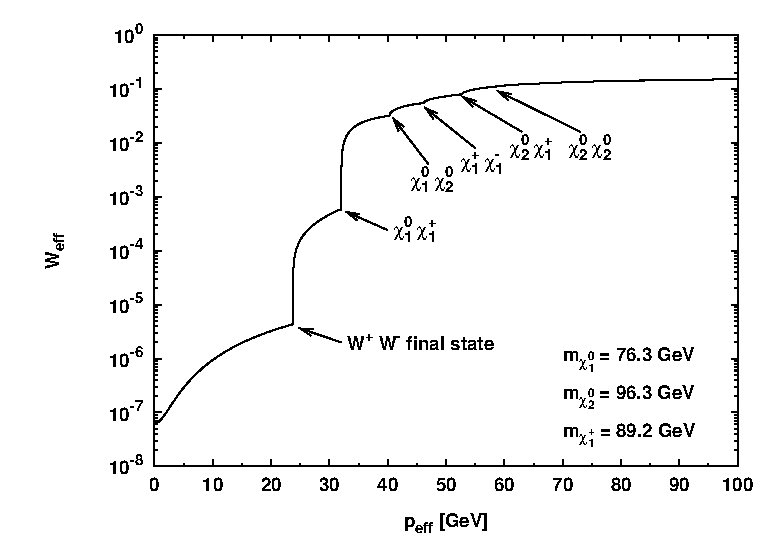
\epsfig{file=fig/rateex.eps,width=0.75\textwidth}}
  \caption{The effective invariant annihiliation rate $W_{\rm eff}$
    as a function of $p_{\rm eff}$ for an example model. 
    The final state threshold for
    annihilation into $W^+ W^-$ and the coannihilation thresholds, as
    given by Eq.~(\protect\ref{eq:weff}), are indicated.  
    The $\chi_2^0 \chi_2^0$ coannihilation threshold is too small to
    be seen.}
  \label{fig:effrate}
\end{figure}

In the effective annihilation rate, coannihilations appear
as thresholds at $\sqrt{s}$ equal to the sum of the masses of the
coannihilating particles.  We show an example in
Fig.~\ref{fig:effrate} where it is clearly seen that the
coannihilation thresholds appear in the effective invariant rate
just as final state thresholds do.  For the same example,
Fig.~\ref{fig:k1effrate} shows the differential annihilation rate
per unit volume $dA/dp_{\rm eff}$, the integrand in
Eq.~(\ref{eq:Apeff}), as a function of $p_{\rm eff}$. We have
chosen a temperature $T=m_{\chi}/20$, a typical freeze-out
temperature. The Boltzmann suppression contained in the exponential
decay of $K_{1}$ at high $p_{\rm eff}$ is clearly visible.  At
higher temperatures the peak shifts to the right and at lower
temperatures to the left.  For the particular model shown in
Figs.~\ref{fig:effrate}--\ref{fig:k1effrate}, the relic density
results $\Omega_\chi h^2=0.030$ when coannihilations are included
and $\Omega_\chi h^2=0.18$ when they are not. Coannihilations
have lowered $\Omega_\chi h^2$ by a factor of 6.

\begin{figure}
  \centerline{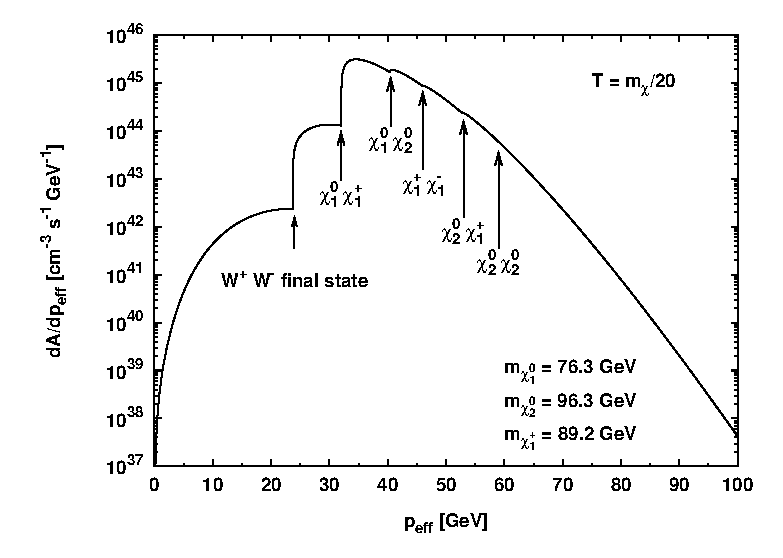
\epsfig{file=fig/k1rateex.eps,width=0.75\textwidth}}
  \caption{Total differential annihilation rate per unit volume 
    $dA/dp_{\rm eff}$ for the same model as in
    Fig.~\protect\ref{fig:effrate}, evaluated at a temperature
    $T=m_\chi/20$, typical of freeze-out. Notice the Boltzmann
    suppression at high $p_{\rm eff}$.}
  \label{fig:k1effrate}
\end{figure}

%%%%%%%%%%%%%%%%%%%%%%%%%%%%%%%%%%%%%%%%%%%%%%%%%%%%%%%%%%%%
\subsection{Internal degrees of freedom}
\label{sec:dof}

If we look at Eqs.~(\ref{eq:weff}) and (\ref{eq:sigmavefffin2}) we see
that we have a freedom on how to treat particles degenerate in mass,
e.g.\ a chargino can be treated either 
\begin{enumerate}
\item[a)]
  as two separate species
  $\chi_{i}^+$ and $\chi_{i}^-$, each with internal degrees of freedom
  $g_{\chi^+}=g_{\chi^-}=2$, or,
\item[b)]
  as a single species
  $\chi_{i}^\pm$ with $g_{\chi_{i}^\pm}=4$ internal degrees of freedom. 
\end{enumerate}
Of course the two views are equivalent, we just have to be careful 
including the $g_{i}$'s consistently whichever view we take.
In a), we have the advantage that all the $W_{ij}$ that enter into 
Eq.~(\ref{eq:weff}) enter as they are, i.e.\ without any correction 
factors for the degrees of freedom. On the other hand we get many 
terms in the sum that are identical and we need some book-keeping 
machinery to avoid calculating identical terms more than once. On the 
other hand, with option b), the sum over $W_{ij}$ in Eq.~(\ref{eq:weff}) 
is much simpler only containing terms that are not identical (except 
for the trivial identity $W_{ij}=W_{ji}$ which is easily taken care of). 
However, the individual $W_{ij}$ will be some linear combinations of 
the more basic $W_{ij}$ entering in option a), where the coefficients 
have to be calculated for each specific type of initial condition. 

Below we will perform this calculation to show how the $W_{ij}$ look 
like in option b) for different initial states. We will use a prime on 
the $W_{ij}$ when they refer to these combined states to indicate the 
difference.

%%%%%
\subsubsection{Neutralino-chargino annihilation}

The starting point is Eq.~(\ref{eq:weff}) which we will use to define 
the $W_{ij}$ in option b) such that $W_{\rm eff}$ is the same as in 
option a). Eq.~(\ref{eq:sigmavefffin2}) is then guaranteed to be the 
same in both cases since the sum in the denominator is linear in $g_{i}$.

Now consider annihilation between $\chi_{i}^0$ and $\chi_{c}^+$ or 
$\chi_{c}^-$. The corresponding terms in Eq.~(\ref{eq:weff}) does for 
option a) read
\begin{eqnarray}
    W_{\rm eff} & = & \sum_{ij}\frac{p_{ij}}{p_{11}} 
    \frac{g_{i}g_{j}}{g_{1}^2} W_{ij}
    =
    \frac{p_{ic}}{p_{11}} \frac{2 \cdot 2}{2^2}
    \bigg[ 
    W_{\chi_{i}^0 \chi_{c}^+} +
    W_{\chi_{i}^0 \chi_{c}^-} +
    \underbrace{W_{\chi_{c}^+ \chi_{i}^0}}_{W_{\chi_{i}^0 \chi_{c}^+}} +
    \underbrace{W_{\chi_{c}^- \chi_{i}^0}}_{W_{\chi_{i}^0 \chi_{c}^-}}
    \bigg] \nonumber \\
    & = & 2 \frac{p_{ic}}{p_{11}} 
    \bigg[
    W_{\chi_{i}^0 \chi_{c}^+} +
    \underbrace{W_{\chi_{i}^0 \chi_{c}^-}}_{W_{\chi_{i}^0 \chi_{c}^+}}
    \bigg]
    = 4 \frac{p_{ic}}{p_{11}} 
    W_{\chi_{i}^0 \chi_{c}^+}
    \label{eq:weffneucha-a}
\end{eqnarray}

For option b), we instead get
\begin{equation}
    W_{\rm eff} = \sum_{ij}\frac{p_{ij}}{p_{11}} 
    \frac{g_{i}g_{j}}{g_{1}^2} W_{ij}
    =
    \frac{p_{ic}}{p_{11}} \frac{2 \cdot 4}{2^2}
    \bigg[ 
    W'_{\chi_{i}^0 \chi_{c}^\pm} +
    \underbrace{W'_{\chi_{c}^\pm \chi_{i}^0}}_{W'_{\chi_{i}^0 \chi_{c}^\pm}}
    \bigg]
    =
    4 \frac{p_{ic}}{p_{11}} W'_{\chi_{i}^0 \chi_{c}^\pm}
    \label{eq:weffneucha-b}
\end{equation}
Comparing Eq.~(\ref{eq:weffneucha-b}) and Eq.~(\ref{eq:weffneucha-a}) 
we see that they are indentical if we make the identification
\begin{equation}
    W'_{\chi_{i}^0 \chi_{c}^\pm} \equiv W_{\chi_{i}^0 \chi_{c}^+}
\end{equation}

%%%%%
\subsubsection{Chargino-chargino annihilation}

First consider the case where we include the terms in the sum for 
which we have annihilation between $\chi_{c}^+$ or $\chi_{c}^-$ and 
$\chi_{d}^+$ or $\chi_{d}^-$ with $c \ne d$.

In option a), the corresponding terms in Eq.~(\ref{eq:weff}) reads
\begin{eqnarray}
    W_{\rm eff} & = & \sum_{ij}\frac{p_{ij}}{p_{11}} 
    \frac{g_{i}g_{j}}{g_{1}^2} W_{ij} \nonumber \\
    & = &
    \frac{p_{cd}}{p_{11}} \frac{2 \cdot 2}{2^2}
    \bigg[ 
    W_{\chi_{c}^+ \chi_{d}^+} +
    W_{\chi_{c}^+ \chi_{d}^-} +
    W_{\chi_{c}^- \chi_{d}^+} +
    W_{\chi_{c}^- \chi_{d}^-} \nonumber \\
    & & +
    \underbrace{W_{\chi_{d}^+ \chi_{c}^+}}_{W_{\chi_{c}^+ \chi_{d}^+}} +
    \underbrace{W_{\chi_{d}^+ \chi_{c}^-}}_{W_{\chi_{c}^- \chi_{d}^+}} +
    \underbrace{W_{\chi_{d}^- \chi_{c}^+}}_{W_{\chi_{c}^+ \chi_{d}^-}} +
    \underbrace{W_{\chi_{d}^- \chi_{c}^-}}_{W_{\chi_{c}^- \chi_{d}^-}}
    \bigg] \nonumber \\
    & = & 
    2 \frac{p_{cd}}{p_{11}}
    \bigg[
    W_{\chi_{c}^+ \chi_{d}^+} +
    W_{\chi_{c}^+ \chi_{d}^-} +
    \underbrace{W_{\chi_{c}^- \chi_{d}^+}}_{W_{\chi_{c}^+ \chi_{d}^-}} +
    \underbrace{W_{\chi_{c}^- \chi_{d}^-}}_{W_{\chi_{c}^+ \chi_{d}^+}}
    \bigg] \nonumber \\
    & = & 
    4 \frac{p_{cd}}{p_{11}}
    \bigg[
    W_{\chi_{c}^+ \chi_{d}^+} +
    W_{\chi_{c}^+ \chi_{d}^-}
    \bigg]
    \label{eq:weffchacha-a}
\end{eqnarray}
In option b), the corresponding terms would instead read
\begin{equation}
    W_{\rm eff} = \sum_{ij}\frac{p_{ij}}{p_{11}} 
    \frac{g_{i}g_{j}}{g_{1}^2} W'_{ij} =
    \frac{p_{cd}}{p_{11}} \frac{4 \cdot 4}{2^2}
    \bigg[ 
    W'_{\chi_{c}^\pm \chi_{d}^\pm} +
    \underbrace{W'_{\chi_{d}^\pm \chi_{c}^\pm}}_{W'_{\chi_{c}^\pm \chi_{d}^\pm}}
    \bigg]
     = 8 \frac{p_{cd}}{p_{11}} W'_{\chi_{c}^\pm \chi_{d}^\pm}
    \label{eq:weffchacha-b}
\end{equation}
Comparing Eq.~(\ref{eq:weffchacha-a}) and Eq.~(\ref{eq:weffchacha-b}) 
we see that they are identical if we make the following identifcation
\begin{equation}
    W'_{\chi_{c}^\pm \chi_{d}^\pm} \equiv \frac{1}{2} 
        \bigg[
    W_{\chi_{c}^+ \chi_{d}^+} +
    W_{\chi_{c}^+ \chi_{d}^-}
    \bigg]
\end{equation} 

For clarity, let's also consider the case where $c=d$.
In option a), the terms in $W_{\rm eff}$ are
\begin{eqnarray}
    W_{\rm eff} & = & \sum_{ij}\frac{p_{ij}}{p_{11}} 
    \frac{g_{i}g_{j}}{g_{1}^2} W_{ij}
    =
    \frac{p_{cc}}{p_{11}} \frac{2 \cdot 2}{2^2}
    \bigg[ 
    W_{\chi_{c}^+ \chi_{c}^+} +
    W_{\chi_{c}^+ \chi_{c}^-} +
    \underbrace{W_{\chi_{c}^- \chi_{c}^+}}_{W_{\chi_{c}^+ \chi_{c}^-}} +
    \underbrace{W_{\chi_{c}^- \chi_{c}^-}}_{W_{\chi_{c}^+ \chi_{c}^+}}
    \bigg] 
    \nonumber \\
    & = &
    2 \frac{p_{cc}}{p_{11}}
    \bigg[
    W_{\chi_{c}^+ \chi_{c}^+} +
    W_{\chi_{c}^+ \chi_{c}^-}
    \bigg]
    \label{eq:weffchacha-a-ident}
\end{eqnarray}
In option b), the corresponding term would instead read
\begin{equation}
    W_{\rm eff} = \sum_{ij}\frac{p_{ij}}{p_{11}} 
    \frac{g_{i}g_{j}}{g_{1}^2} W'_{ij} =
    \frac{p_{cc}}{p_{11}} \frac{4 \cdot 4}{2^2}
    W'_{\chi_{c}^\pm \chi_{c}^\pm} +
     = 4 \frac{p_{cc}}{p_{11}} W'_{\chi_{c}^\pm \chi_{c}^\pm}
    \label{eq:weffchacha-b-ident}
\end{equation}
Comparing Eq.~(\ref{eq:weffchacha-a-ident}) and 
Eq.~(\ref{eq:weffchacha-b-ident}) 
we see that they are identical if we make the following identifcation
\begin{equation}
    W'_{\chi_{c}^\pm \chi_{c}^\pm} \equiv \frac{1}{2} 
        \bigg[
    W_{\chi_{c}^+ \chi_{c}^+} +
    W_{\chi_{c}^+ \chi_{c}^-}
    \bigg]
\end{equation} 
i.e.\ the same identification as in the case $c \ne d$.

%%%%%
\subsubsection{Neutralino-sfermion annihilation}

For each sfermion we have in total four different states,
$\tilde{f}_{1}$, $\tilde{f}_{2}$, $\tilde{f}_{1}^{*}$ and
$\tilde{f}_{2}^{*}$.  Of these, the $\tilde{f}_{1}$ and
$\tilde{f}_{2}$ in general have different masses and have to be treated
separately.  Considering only one mass eigenstate $\tilde{f}_{k}$,
option a) then means that we treat $\tilde{f}_{k}$ and
$\tilde{f}_{k}^{*}$ as two separate species with $g_{i}=1$ degree of
freedom each, whereas option b) means that we treat them as one
species $\tilde{f}'_{k}$ with $g_{i}=2$ degrees of freedom.  As
before, the prime indicates that we mean both the particle and the
antiparticle state.

Note, that for squarks we also have the number of colours $N_c=3$ to take into account.
In option a) we should choose to treat even colour state differently, i.e.\ $g_i=1$, whereas $g_i=6$ in case b). 
The expressions would be the same as above except that both the expression in a) and b) would be multiplied by the colour factor $N_c=3$. The expression relating case a) and case b) is thus unaffected by this colour factor. Note however, that in option b) we take the average over the squark colours (or in this case calculate it only for one colour. See sections \ref{sec:sqsq} and \ref{sec:sfsq} below for more details.

For option a), Eq.~(\ref{eq:weff}) then reads
\begin{eqnarray}
    W_{\rm eff} & = & \sum_{ij}\frac{p_{ij}}{p_{11}} 
    \frac{g_{i}g_{j}}{g_{1}^2} W_{ij}
    =
    \frac{p_{ik}}{p_{11}} \frac{2 \cdot 1}{2^2}
    \bigg[ 
    W_{\chi_{i}^0 \tilde{f}_{k}} +
    W_{\chi_{i}^0 \tilde{f}_{k}^*} +
    \underbrace{W_{\tilde{f}_{k} \chi_{i}^0}}_{W_{\chi_{i}^0 \tilde{f}_{k}}} +
    \underbrace{W_{\tilde{f}_{k}^{*} \chi_{i}^0}}_{W_{\chi_{i}^0 \tilde{f}_{k}^*}}
    \bigg] 
    \nonumber \\
    & = &
    \frac{p_{ik}}{p_{11}}
    \bigg[
    W_{\chi_{i}^0 \tilde{f}_{k}} +
    \underbrace{W_{\chi_{i}^0 \tilde{f}_{k}^*}}_{W_{\chi_{i}^0 \tilde{f}_{k}}}
    \bigg]
    =
    2 \frac{p_{ik}}{p_{11}}
    W_{\chi_{i}^0 \tilde{f}_{k}}
    \label{eq:weffneusf-a}
\end{eqnarray}
whereas for option b), Eq.~(\ref{eq:weff}) reads
\begin{equation}
    W_{\rm eff} = \sum_{ij}\frac{p_{ij}}{p_{11}} 
    \frac{g_{i}g_{j}}{g_{1}^2} W'_{ij}
    =
    \frac{p_{ik}}{p_{11}} \frac{2 \cdot 2}{2^2}
    \bigg[ 
    W'_{\chi_{i}^0 \tilde{f'}_{k}} +
    \underbrace{W'_{\tilde{f'}_{k} \chi_{i}^0}}_{W'_{\chi_{i}^0 \tilde{f'}_{k}}}
    \bigg] 
    =
    2 \frac{p_{ik}}{p_{11}}
    W'_{\chi_{i}^0 \tilde{f'}_{k}}
    \label{eq:weffneusf-b}
\end{equation}
Comparing Eq.~(\ref{eq:weffneusf-b}) and Eq.~(\ref{eq:weffneusf-a}) we 
see that they are indentical if we make the identification
\begin{equation}
    W'_{\chi_{i}^0 \tilde{f'}_{k}} \equiv W_{\chi_{i}^0 \tilde{f}_{k}}
\end{equation}

For clarity, for squarks the corresponding expression would be
\begin{equation}
    W'_{\chi_{i}^0 \tilde{q'}_{k}} \equiv
   \frac{1}{3}\sum_{a=1}^3 W_{\chi_{i}^0 \tilde{q}_{k}^a}
\end{equation}
where $a$ is a colour index.

%%%%%
\subsubsection{Chargino-sfermion annihilation}

In option a) the chargino has $g_i=2$ and the sfermion has $g_i=1$ degrees of freedom, whereas in option b), the chargino has $g_i=4$ and the sfermion has $g_i=2$ degrees of freedom

For option a), Eq.~(\ref{eq:weff}) then reads
\begin{eqnarray}
    W_{\rm eff} & = & \sum_{ij}\frac{p_{ij}}{p_{11}} 
    \frac{g_{i}g_{j}}{g_{1}^2} W_{ij} \nonumber \\
    & = &
    \frac{p_{ck}}{p_{11}} \frac{2 \cdot 1}{2^2}
    \bigg[ 
    W_{\chi_{c}^+ \tilde{f}_{k}} +
    W_{\chi_{c}^+ \tilde{f}_{k}^*} +
    W_{\chi_{c}^- \tilde{f}_{k}} +
    W_{\chi_{c}^- \tilde{f}_{k}^*} \nonumber \\
    & & +
    \underbrace{W_{\tilde{f}_{k} \chi_{c}^+}}_
      {W_{\chi_{c}^+ \tilde{f}_{k}}} +
    \underbrace{W_{\tilde{f}_{k}^* \chi_{c}^+}}_
      {W_{\chi_{c}^+ \tilde{f}_{k}^*}} +
    \underbrace{W_{\tilde{f}_{k} \chi_{c}^-}}_
      {W_{\chi_{c}^- \tilde{f}_{k}}} +
    \underbrace{W_{\tilde{f}_{k}^* \chi_{c}^-}}_
      {W_{\chi_{c}^- \tilde{f}_{k}^*}}
    \bigg] \nonumber \\
    & = &
    \frac{p_{ck}}{p_{11}}
    \bigg[ 
    W_{\chi_{c}^+ \tilde{f}_{k}} +
    W_{\chi_{c}^+ \tilde{f}_{k}^*} +
    \underbrace{W_{\chi_{c}^- \tilde{f}_{k}}}_
      {W_{\chi_{c}^+ \tilde{f}_{k}^*}} +
    \underbrace{W_{\chi_{c}^- \tilde{f}_{k}^*}}_
      {W_{\chi_{c}^+ \tilde{f}_{k}}}
    \bigg]
    = 
    2 \frac{p_{ck}}{p_{11}}
    \bigg[ 
    W_{\chi_{c}^+ \tilde{f}_{k}} +
    W_{\chi_{c}^+ \tilde{f}_{k}^*} \bigg]
    \label{eq:weffchasf-a}
\end{eqnarray}

In option b), Eq.~(\ref{eq:weff}) reads
\begin{eqnarray}
    W_{\rm eff} & = & \sum_{ij}\frac{p_{ij}}{p_{11}} 
    \frac{g_{i}g_{j}}{g_{1}^2} W'_{ij}
    =
    \frac{p_{ck}}{p_{11}} \frac{4 \cdot 2}{2^2}
    \bigg[ 
    W'_{\chi_{c}^\pm \tilde{f'}_{k}} +
    \underbrace{W'_{\tilde{f'}_{k} \chi_{c}^\pm}}_
      {W'_{\chi_{c}^\pm \tilde{f'}_{k}}} \bigg]
    = 4 \frac{p_{ck}}{p_{11}} W'_{\chi_{c}^\pm \tilde{f'}_{k}}
    \label{eq:weffchasf-b}
\end{eqnarray}

Comparing Eq.~(\ref{eq:weffchasf-b}) and Eq.~(\ref{eq:weffchasf-a}) we 
see that they are indentical if we make the identification
\begin{equation}
    W'_{\chi_{c}^\pm \tilde{f'}_{k}} \equiv
    \frac{1}{2} \bigg[ 
    W_{\chi_{c}^+ \tilde{f}_{k}} + 
    W_{\chi_{c}^+ \tilde{f}_{k}^*}
    \bigg] 
\end{equation}

For clarity, for squarks the corresponding expression would be
\begin{equation}
    W'_{\chi_{c}^\pm \tilde{q'}_{k}} \equiv
    \frac{1}{2} \frac{1}{3}\sum_{a=1}^3 \bigg[ 
    W_{\chi_{c}^+ \tilde{q}_{k}^a} + 
    W_{\chi_{c}^+ \tilde{q}_{k}^{a*}}
    \bigg] 
\end{equation}
where $a$ is a colour index.


%%%%%
\subsubsection{Sfermion-sfermion annihilation}

First consider the case where we have annihilation between sfmerions 
of different types, i.e.\ annihilation between $\tilde{f}_{k}$ or 
$\tilde{f}_{k}^{*}$ and $\tilde{f}_{l}$ or $\tilde{f}_{l}^{*}$.

For option a), Eq.~(\ref{eq:weff}) then reads
\begin{eqnarray}
    W_{\rm eff} & = & \sum_{ij}\frac{p_{ij}}{p_{11}} 
    \frac{g_{i}g_{j}}{g_{1}^2} W_{ij}
    \nonumber \\
    & = & \frac{p_{kl}}{p_{11}} \frac{1 \cdot 1}{2^2}
    \bigg[ 
    W_{\tilde{f}_{k} \tilde{f}_{l}} +
    W_{\tilde{f}_{k} \tilde{f}_{l}^{*}} +
    W_{\tilde{f}_{k}^{*} \tilde{f}_{l}} +
    W_{\tilde{f}_{k}^{*} \tilde{f}_{l}^{*}} \nonumber \\
    & & +
    \underbrace{W_{\tilde{f}_{l} \tilde{f}_{k}}}_
       {W_{\tilde{f}_{k} \tilde{f}_{l}}} +
    \underbrace{W_{\tilde{f}_{l} \tilde{f}_{k}^{*}}}_
       {W_{\tilde{f}_{k}^{*} \tilde{f}_{l}}} +
    \underbrace{W_{\tilde{f}_{l}^{*} \tilde{f}_{k}}}_
       {W_{\tilde{f}_{k} \tilde{f}_{l}^{*}}} +
    \underbrace{W_{\tilde{f}_{l}^{*} \tilde{f}_{k}^{*}}}_
       {W_{\tilde{f}_{k}^{*} \tilde{f}_{l}^{*}}}
    \bigg]  \nonumber \\
    & = &
    \frac{1}{2} \frac{p_{kl}}{p_{11}}
    \bigg[ 
    W_{\tilde{f}_{k} \tilde{f}_{l}} +
    W_{\tilde{f}_{k} \tilde{f}_{l}^{*}} +
    \underbrace{W_{\tilde{f}_{k}^{*} \tilde{f}_{l}}}_
        {W_{\tilde{f}_{k} \tilde{f}_{l}^{*}}} +
    \underbrace{W_{\tilde{f}_{k}^{*} \tilde{f}_{l}^{*}}}_
        {W_{\tilde{f}_{k} \tilde{f}_{l}}}
    \bigg] 
    = \frac{p_{kl}}{p_{11}}
    \bigg[ 
    W_{\tilde{f}_{k} \tilde{f}_{l}} +
    W_{\tilde{f}_{k} \tilde{f}_{l}^{*}}
    \bigg] \label{eq:weffsfsf-a}
\end{eqnarray}    

In option b) we would get 
\begin{eqnarray}
    W_{\rm eff} & = & \sum_{ij}\frac{p_{ij}}{p_{11}} 
    \frac{g_{i}g_{j}}{g_{1}^2} W'_{ij}
    \nonumber \\
    & = & \frac{p_{kl}}{p_{11}} \frac{2 \cdot 2}{2^2}
    \bigg[ 
    W'_{\tilde{f'}_{k} \tilde{f'}_{l}} +
    \underbrace{W'_{\tilde{f'}_{l} \tilde{f'}_{k}}}_
       {W'_{\tilde{f'}_{k} \tilde{f'}_{l}}} \bigg]
    = 2 \frac{p_{kl}}{p_{11}} \bigg[
    W'_{\tilde{f'}_{k} \tilde{f'}_{l}}\bigg]
    \label{eq:weffsfsf-b}
\end{eqnarray}
Comparing Eq.~(\ref{eq:weffsfsf-b}) and Eq.~(\ref{eq:weffsfsf-a}) we 
see that they are indentical if we make the identification
\begin{equation}
    W'_{\tilde{f'}_{k} \tilde{f'}_{l}} \equiv 
    \frac{1}{2} \bigg[
    W_{\tilde{f}_{k} \tilde{f}_{l}} + 
    W_{\tilde{f}_{k} \tilde{f}_{l}^*} \bigg] 
\end{equation}
It is easy to show that this relation holds true even if $k=l$.

%%%%%
\subsubsection{Squark-squark annihilation}
\label{sec:sqsq}

Even though we treated sfermion-sfermion annihilation in the previous subsection, squarks have colour which can complicate things, so let's for clarity consider squarks separately.

Let's denote the squarks $\tilde{q}_k^a$ where $a$ is now a colour index. In option a) we will let each colour be a seprate species, which means that $g_i=1$ in this case. In option b) we will instead have $g_i=6$.

In option a) we would have 
\begin{eqnarray}
    W_{\rm eff} & = & \sum_{ij}\frac{p_{ij}}{p_{11}} 
    \frac{g_{i}g_{j}}{g_{1}^2} W_{ij}
    \nonumber \\
    & = & \frac{p_{kl}}{p_{11}} \frac{1 \cdot 1}{2^2}
    \sum_{a,b=1}^3 \bigg[ 
    W_{\tilde{q}_{k}^a \tilde{q}_{l}^b} +
    W_{\tilde{q}_{k}^a \tilde{q}_{l}^{b*}} +
    W_{\tilde{q}_{k}^{a*} \tilde{q}_{l}^b} +
    W_{\tilde{q}_{k}^{a*} \tilde{q}_{l}^{b*}} \nonumber \\
    & & +
    \underbrace{W_{\tilde{q}_{l}^a \tilde{q}_{k}^b}}_
       {W_{\tilde{q}_{k}^a \tilde{q}_{l}^b}} +
    \underbrace{W_{\tilde{q}_{l}^a \tilde{q}_{k}^{b*}}}_
       {W_{\tilde{q}_{k}^{a*} \tilde{q}_{l}^b}} +
    \underbrace{W_{\tilde{q}_{l}^{a*} \tilde{q}_{k}^b}}_
       {W_{\tilde{q}_{k}^a \tilde{q}_{l}^{b*}}} +
    \underbrace{W_{\tilde{q}_{l}^{a*} \tilde{q}_{k}^{b*}}}_
       {W_{\tilde{q}_{k}^{a*} \tilde{q}_{l}^{b*}}}
    \bigg]  \nonumber \\
    & = &
    \frac{1}{2} \frac{p_{kl}}{p_{11}}
    \sum_{a,b=1}^3 \bigg[ 
    W_{\tilde{q}_{k}^a \tilde{f}_{l}^b} +
    W_{\tilde{q}_{k}^a \tilde{f}_{l}^{b*}} +
    \underbrace{W_{\tilde{q}_{k}^{a*} \tilde{q}_{l}^b}}_
        {W_{\tilde{q}_{k}^a \tilde{q}_{l}^{b*}}} +
    \underbrace{W_{\tilde{q}_{k}^{a*} \tilde{q}_{l}^{b*}}}_
        {W_{\tilde{q}_{k}^a \tilde{q}_{l}^b}}
    \bigg] 
    = \frac{p_{kl}}{p_{11}}
    \sum_{a,b=1}^3 \bigg[ 
    W_{\tilde{q}_{k}^a \tilde{q}_{l}^b} +
    W_{\tilde{q}_{k}^a \tilde{q}_{l}^{b*}}
    \bigg] \label{eq:weffsqsq-a}
\end{eqnarray}    

In option b) we would get 
\begin{eqnarray}
    W_{\rm eff} & = & \sum_{ij}\frac{p_{ij}}{p_{11}} 
    \frac{g_{i}g_{j}}{g_{1}^2} W'_{ij}
    \nonumber \\
    & = & \frac{p_{kl}}{p_{11}} \frac{6 \cdot 6}{2^2}
    \bigg[ 
    W'_{\tilde{q'}_{k} \tilde{q'}_{l}} +
    \underbrace{W'_{\tilde{q'}_{l} \tilde{q'}_{k}}}_
       {W'_{\tilde{q'}_{k} \tilde{q'}_{l}}} \bigg]
    = 18 \frac{p_{kl}}{p_{11}} \bigg[
    W'_{\tilde{q'}_{k} \tilde{q'}_{l}}\bigg]
    \label{eq:weffsqsq-b}
\end{eqnarray}
Comparing Eq.~(\ref{eq:weffsqsq-b}) and Eq.~(\ref{eq:weffsqsq-a}) we 
see that they are indentical if we make the identification
\begin{equation}
    W'_{\tilde{q'}_{k} \tilde{q'}_{l}} \equiv 
    \frac{1}{2} \frac{1}{9}\sum_{a,b=1}^3 \bigg[
    W_{\tilde{q}_{k}^a \tilde{q}_{l}^b} + 
    W_{\tilde{q}_{k}^a \tilde{q}_{l}^{b*}} \bigg] 
\end{equation}
i.e. we get the same relation as for other sfermions, the only difference being that
we in option b) should also take the average over the colour states. 

%%%%%
\subsubsection{Sfermion-squark annihilation}
\label{sec:sfsq}

For clarity, if we have annihilation between a non-coloured sfermion and a squark, we would in the same way as in the previous subsection get
\begin{equation}
    W'_{\tilde{f'}_{k} \tilde{q'}_{l}} \equiv 
    \frac{1}{2} \frac{1}{3}\sum_{b=1}^3 \bigg[
    W_{\tilde{f}_{k} \tilde{q}_{l}^b} + 
    W_{\tilde{f}_{k} \tilde{q}_{l}^{b*}} \bigg] 
\end{equation}


%%%%%
\subsubsection{Summary of degrees of freedom}

We have found above the following relations between option b) and option a),
\begin{equation}
  \left\{ \begin{array}{lcl}
% neutralino-chargino
  W'_{\chi_{i}^0 \chi_{j}^\pm} & \equiv & W_{\chi_{i}^0 \chi_{j}^+} = 
    W_{\chi_{i}^0 \chi_{j}^-} \quad , \quad \forall\ i=1,\ldots,4,\ 
    j=1,2 \anl
% chargino-chargino
  W'_{\chi_{i}^\pm \chi_{j}^\pm} & \equiv & \frac{1}{2} 
  \left[ W_{\chi_{i}^+ \chi_{j}^+} +  
  W_{\chi_{i}^+ \chi_{j}^-}\right] = 
  \frac{1}{2} \left[ W_{\chi_{i}^- \chi_{j}^-} +  
  W_{\chi_{i}^- \chi_{j}^+}\right] \quad , \quad \forall\ i=1,2,\ j=1,2 \anl
% neutralino-sfermion
  W'_{\chi_{i}^0 \tilde{f'}_{k}} & \equiv & W_{\chi_{i}^0 \tilde{f}_{k}}
  \quad , \quad \forall i=1,\ldots 4,\ k=1,2 \anl
% chargino-sfermion
  W'_{\chi_{c}^\pm \tilde{f'}_{k}} & \equiv &
    \frac{1}{2} \left[ 
    W_{\chi_{c}^+ \tilde{f}_{k}} + 
    W_{\chi_{c}^+ \tilde{f}_{k}^*}
    \right]
  \quad , \quad \forall c=1,2,\ k=1,2 \anl
% sfermion-sfmerion
  W'_{\tilde{f'}_{k} \tilde{f'}_{l}} & \equiv & 
    \frac{1}{2} \left[
    W_{\tilde{f}_{k} \tilde{f}_{l}} + 
    W_{\tilde{f}_{k} \tilde{f}_{l}^*} \right] 
  \quad , \quad \forall k=1,2,\ l=1,2 \anl
% squark-squark
  W'_{\tilde{q'}_{k} \tilde{q'}_{l}} & \equiv & 
    \frac{1}{2} \frac{1}{9}\sum_{a,b=1}^3 \left[
    W_{\tilde{q}_{k}^a \tilde{q}_{l}^b} + 
    W_{\tilde{q}_{k}^a \tilde{q}_{l}^{b*}} \right] 
  \quad , \quad \forall k=1,2,\ l=1,2
  \end{array} \right.
\end{equation}
We don't list all the possible cases with squarks explicitly, the principle being that we in option b) should take the \emph{average} over the squark colour states (see the squark-squark entry in the list above).

We will choose option b) and the code (\code{dsandwdcoscn}, \code{dsandwdcoscn}, \code{dsasdwdcossfsf} and \code{dsasdwdcossfchi}) should thus return $W'$ as defined above. Note again that squarks are assumed to have $g_i=6$ degrees of freedom in this convention and the summing over colours should also be taken into account in the code.


%%%%%%%%%%%%%%%%%%%%%%%%%%%%%%%%%%%%%%
\subsection{Reformulation of the Boltzmann equation}

We now follow Gondolo and Gelmini \cite{GondoloGelmini} to 
put Eq.~(\ref{eq:Boltzmann2}) in a more convenient form by
considering the ratio of the number density to the entropy density,
\begin{equation} \label{eq:ydef}
  Y = \frac{n}{s}.
\end{equation}
Consider
\begin{equation}
  \frac{dY}{dt} = \frac{d}{dt} \left( \frac{n}{s} \right) = 
  \frac{\dot{n}}{s}-\frac{n}{s^2}\dot{s}
\end{equation}
where dot means time derivative. In absence
of entropy production, $S=R^3s$ is constant ($R$ is the scale factor).
Differentiating with respect to time we see 
that
\begin{equation}
  \dot{s} = -3\frac{\dot{R}}{R} s = -3Hs
\label{eq:entropycons}
\end{equation}
which yields
\begin{equation}
  \dot{Y} = \frac{\dot{n}}{s} + 3H \frac{n}{s}.
\end{equation}
Hence we can rewrite Eq.~(\ref{eq:Boltzmann2}) as
\begin{equation} \label{eq:Boltzmann3}
  \dot{Y} = -s  \langle \sigma_{\rm{eff}} v \rangle 
  \left( Y^2 - Y_{\rm{eq}}^2 \right).
\end{equation}

The right-hand side depends only on temperature, and it is therefore
convenient to use temperature $T$ instead of time $t$ as independent
variable. Defining $x=m_1/T$ we have
\begin{equation}
  \frac{dY}{dx} = - \frac{m_{1}}{x^2} \frac{1}{3H} \frac{ds}{dT}
  \langle \sigma_{\rm{eff}} v \rangle \left( Y^2 -
  Y_{\rm{eq}}^2 \right).
\label{eq:Boltzmann3bis}
\end{equation}
where we have used
\begin{equation}
  \frac{1}{\dot{T}} = \frac{1}{\dot{s}} \frac{ds}{dT} = -
  \frac{1}{3Hs} \frac{ds}{dT} 
\end{equation} 
which follows from Eq.~(\ref{eq:entropycons}). 
With the Friedmann equation in a radiation dominated universe
\begin{equation}
  H^2 = \frac{8\pi G \rho}{3} ,
\end{equation}
where $G$ is the gravitational constant, and the
usual parameterization of the energy and entropy densities
in terms of the effective degrees of freedom $g_{\rm{eff}}$ and
$h_{\rm{eff}}$, \begin{equation} \label{eq:geffheff}
  \rho = g_{\rm{eff}}(T) \frac{\pi^2}{30} T^4
  , \quad 
  s = h_{\rm{eff}}(T) \frac{2\pi^2}{45} T^3 ,
\end{equation}
we can cast Eq.~(\ref{eq:Boltzmann3bis})
into the form \cite{GondoloGelmini}
\begin{equation} \label{eq:Boltzmann4}
  \frac{dY}{dx} = - \sqrt{\frac{\pi}{45G}} \frac{g_{*}^{1/2}m_1}{x^2}
  \langle \sigma_{\rm{eff}} v \rangle \left( Y^2 -
  Y_{\rm{eq}}^2 \right) 
\end{equation}
where $Y_{\rm eq}$ can be written as
\begin{equation}
  Y_{\rm{eq}} = \frac{n_{\rm{eq}}}{s} = 
  \frac{45 x^2}{4 \pi^4 h_{\rm{eff}}(T)} \sum_i g_i
  \left( \frac{m_i}{m_1} \right)^2 K_{2} \left( x 
\frac{m_{i}}{m_1}\right),
\end{equation}
using Eqs.~(\ref{eq:neq}), (\ref{eq:ydef}) and
(\ref{eq:geffheff}).

The parameter $g_{*}^{1/2}$ is defined as
\begin{equation}
  g_{*}^{1/2} = \frac{h_{\rm{eff}}}{\sqrt{g_{\rm{eff}}}}
  \left( 1+\frac{T}{3h_{\rm{eff}}} \frac{d h_{\rm{eff}}}{dT}
  \right)
\end{equation}

For $g_{\rm eff}$, $h_{\rm eff}$ and $g_*^{1/2}$ \ds\ has the option of either using the results of Gondolo and Gelmini \cite{GondoloGelmini} with a QCD phase-transition
temperature $T_{QCD} = 150 $ MeV or the later results of Hindmarsh and Philipsen \cite{hp05}. The default in \ds\ is to use the results for equation of state B in Hindmarsh and Philipsen. The user can change this default choice with a call to \code{dsrdset} (see header of that file for explanation of how to call it).
Using the Hindmarsh and Philipsen equation of state B (default) gives about 1.5--3.5\% higher relic densities than the Gondolo and Gelmini degrees of freedom.

%Our results are insensitive to the
%value of $T_{QCD}$, because due to a lower limit on the neutralino
%mass the neutralino freeze-out temperature is always much larger
%than $T_{QCD}$.

To obtain the relic density we integrate Eq.~(\ref{eq:Boltzmann4})
from $x=0$ to $x_0=m_\chi/T_0$ where $T_0$ is the photon temperature
of the Universe today. The relic density today in units of the
critical density is then given by
\begin{equation}
  \Omega_\chi = \rho_\chi^0/\rho_{\rm
  crit}=m_\chi s_0 Y_0/\rho_{\rm crit}
\end{equation}
where $\rho_{\rm crit}=3 H^2/8 \pi G$ is the critical density, $s_{0}$ 
is the entropy density today and $Y_{0}$ is the result of the 
integration of Eq.~(\ref{eq:Boltzmann4}). With a
background radiation temperature of $T_0=2.726$ K we finally obtain
\begin{equation} \label{eq:omegah2}
  \Omega_\chi h^2 = 2.755\times 10^8 \frac{m_\chi}{\mbox{GeV}} Y_0.
\end{equation}

